\subsection{Changes to accessibility settings}
A decision was made to create a feature which could add a pictogram to specific users in the system. 
Previously we have the option of assigning the pictogram to the user, as private, or available to everyone, as public.

We changed the public to be institution wide, meaning the pictogram was available to the members of the institution.
The private option was changed to be available for specific citizens, chosen from a list which contains the citizens assigned to the currently logged in guardian.
To avoid confusion, it was decided that the button to add citizens and the list with the citizens would be hidden until the user checks the citizen button.

This change required a significant overhaul in the GUI of the save dialogue, the resulting GUI can be seen in \figref{fig:save_dialogue2}, where the citizen button is checked and two citizens are chosen.

\begin{figure}[h]
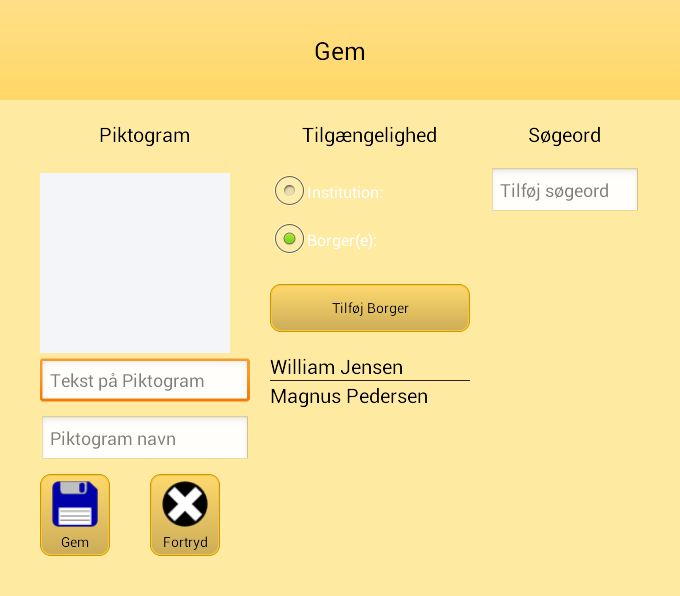
\includegraphics[scale=0.5]{media/sprint4/save_dialog2}
\caption{Example showing the button where citizen can be given access to a pictogram.}
\label{fig:save_dialogue2}
\end{figure}

When the button \textit{Tilføj Borger} is clicked a new dialogue will show up where the citizens can be clicked, as seen in \figref{fig:save_dialogue3}, where the darker fields are chosen whereas the light is not.
The dialogue is a component from the GUI library created by the GUI group in the multi-project.
The text colour on the radio buttons are white due to the library, but should have been black as they are not clearly visible.

\begin{figure}[h]
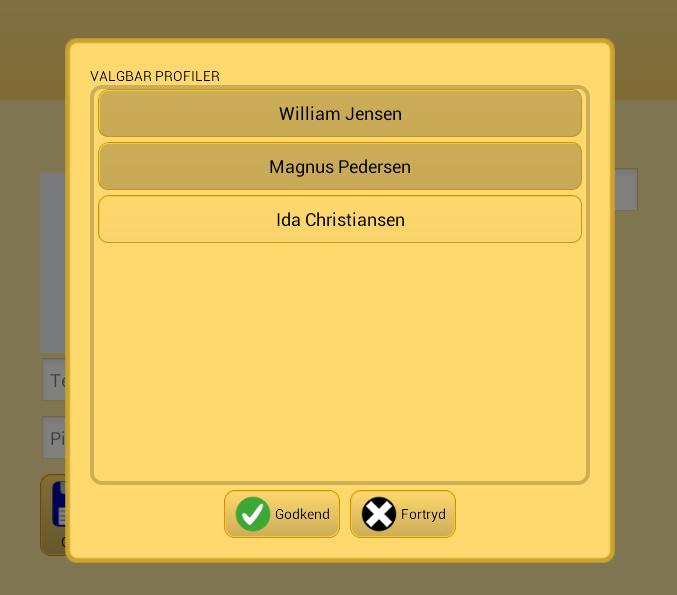
\includegraphics[scale=0.5]{media/sprint4/save_dialog3}
\caption{The dialogue where citizen are chosen for access.}
\label{fig:save_dialogue3}
\end{figure}
